\documentclass[../main.tex]{subfiles}
\begin{document}

\tags{
    \nameref{hc:dataviz},
    \nameref{hc:correlation},
    \nameref{hc:medium},
    \nameref{hc:professionalism},
    \nameref{hc:testability}
}{
    None
}

\vspace{\baselineskip}

This chapter presents results and analyses aimed at validating the approach and the implementation of the Maccabee package. The content is split into two sections corresponding to the two aspects of Maccabee's design which require careful validation. The first section presents results aimed at validating the DGP sampling parameterization by showing that Maccabee is able to sample DGPs from specified locations in the distributional problem space. The second section presents the results aimed at validating the benchmarking approach by looking at a number of applicable case studies. Demos and examples presented throughout the \href{\RTDurl/usage.html}{tutorials} in the package documentation validate the basic operational correctness of the benchmarking code.

\vspace{\baselineskip}

It is worth noting, explicitly, that validating this package with any level of certainty is a hard problem. First, and most generally, because there is no good way to objectively and quantitatively compare different benchmarking approaches. Producing different results for some method relative to other benchmarking approaches is not indicative of either success/failure without a deeper understanding of why the results differ. Second, as the reader will see below, validating the Maccabee approach relies on quantifying the position of sampled DGPs in the distributional problem space by using a set of \textit{data metrics} that were introduced in Chapter \ref{chap:problemspace}. These metrics are noisy/imprecise measurements of the true distributional setting of a DGP. In fact, \textcite{Dorie2019Automated1} find almost no correlation between the metrics they propose (the same ones used in this work) and estimator performance even though estimator performance is strongly correlated with the parameterization that they used to control distributional setting in their paper. This means the changes in the distributional setting created by different parameterization of the DGP sampling process are not clearly reflected in changes in the value of metrics. The first section below relies, unavoidably, on the metrics. However, in the second section, I have made an effort to define a validation scheme that is not overly reliant on the metric values.

\section{Validating the DGP Sampling Parameterization}
\label{sec:validation-dgp-sampling}

Chapter \ref{chap:macdesign} established that one of Maccabee's key design goals is to allow the sampling of DGPs from specified locations in the distributional problem space through the use of a parameterized DGP sampling procedure. Chapter \ref{chap:macimplementation}, and the documentation linked therein, discussed the different ways in which the parameters of the sampling process can be specified by the user. These can be summarized as either \textit{preset} - specifying parameters by selecting a \textit{high}, \textit{medium} or \textit{low} level on each supported axis of the problem space and using the low-level parameter values built into the package. Or, \textit{customized} - specifying the low-level parameters directly. This section focuses on validating the first approach. If custom low-level parameters are required, users should follow the advanced tutorials in the \RTDlink{package documentation} in order to refine parameter values using the relevant data metrics.

\vspace{\baselineskip}

Figure \ref{fig:sampling-validation-results-1} displays the primary DGP sampling validation results. Each subplot corresponds to a single axis of the problem space. The Y-axis is the value of a metric that measures the location of sampled DGPs along the problem space axis and the X-axis is the user-specified target \textit{level} for the axis. In each plot, the parameters corresponding to all other axis are kept at package default values. The metric value at each level is evaluated by sampling 32 DGPs and then sampling 100 datasets from each DGP. The value of the data metric is averaged across the datasets for each DGP and then averaged across all DGPs. The error bars correspond to the standard deviation of the metric value between DGPs.

\begin{figure}[ht!]
    \centering
    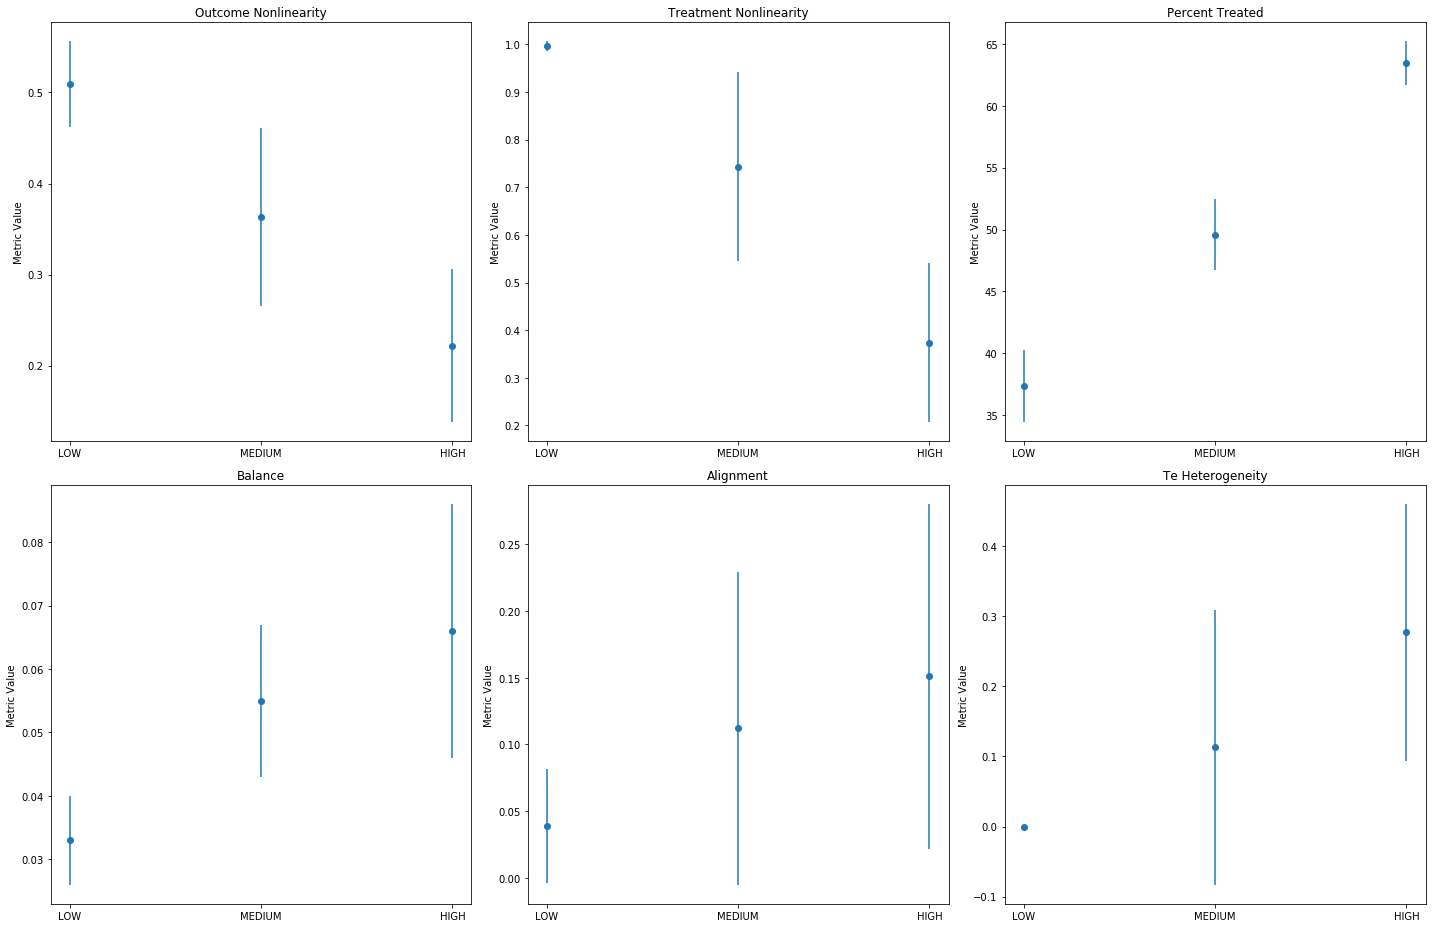
\includegraphics[width=1\linewidth]{figures/ch7-sampling-validation-1.png}
    \caption{DGP sampling parameterization results - metric values for each axis when DGPs are sampled at the axis level on the X axis.}
    \label{fig:sampling-validation-results-1}
\end{figure}

The plots indicate that the level-based specification provides for reasonable control over the position of sampled DGPs along each axis. Across all axes, the mean of the metric value at each level increases/decreases in the direction expected given the change in level\footnote{Note that, for each axis, the meaning of low, medium, and high is taken from the natural semantic interpretation of a low, medium and high level of that axis. So, for example, low imbalance means a more imbalanced covariate distribution in the treatment and control group, while a low outcome non-linearity means a more linear outcome mechanism.}. Below, I describe the metric used to measure each value; see Chapter \ref{chap:problemspace} for a thorough theoretical introduction to the construction of these metrics. Working from top left to bottom right:

\begin{itemize}
    \item \textbf{Outcome Non-linearity} measured by the $R^2$ value of a linear regression of the observed outcome on the observed covariates. The value of this metric decreases as the level of the axis is changed from low to high, as would be expected under decreasing linearity of the outcome mechanism.
    
    \item \textbf{Treatment Assignment Nonlinearity} measured by the $R^2$ value of a linear regression of the oracle treatment probability logit on the observed covariates. The value of this metric decreases as the level of the axis is changed from low to high, as would be expected under decreasing linearity of the treatment assignment mechanism.
    
    \item \textbf{Percent Treated} measured by the percent of units in the treated group. The value of this metric increases, as expected, as the percent treated axis level is changed from low to high.
    
    \item \textbf{Imbalance} measured by the Wasserstein Distance\footnote{The Wasserstein Distance is an \textit{integral probability metric} that measures the absolute value of the difference between the CDF of each distribution, integrated across the domain. This can be approximated by formulating a minimum flow optimization problem using the observed covariate values in each group. See the implemented metric code for detailed documentation.} between the covariate distributions in each treatment group. A higher metric value (larger Wasserstein Distance) indicates a larger distance between the distributions in each group, meaning greater imbalance. The values of this metrics increase, as expected, as the imbalance axis level is changed from low balance to high balance. 
    
    \item \textbf{Alignment} measured by a linear regression of the observed outcome on the oracle treatment probability logit. A higher value of the metric means there is greater overlap in covariates between the treatment and outcome mechanisms. The values of the metric increase, as expected, as the alignment axis level is changed from low to high.
    
    \item \textbf{Treatment Effect Heterogeneity} measured by the ratio of the standard deviation of the treatment effect to the standard deviation of the observed outcome. The values of the metric increase as the axis level is changed from low to high, indicating an increasing portion of the individual outcome variance stems from changes in the treatment effect between individuals.
\end{itemize}

Note that, despite the promising trend in the mean of each metric, there is a weakness evident in the plot: The variance of the sampling process appears to be substantial relative to the scale of the differences in metric values at each level. Some of this variance may be equivalent to \textit{measurement} noise\footnote{This noise could stem from the imprecise nature of the metric calculations and the stochasticity of the data sampled from each DGP.} rather than indicating variance in the DGP sampling process itself. This can be tested by increasing the number of samples of data from each DGP to see if the standard deviation of the metric across DGPs decreases. Doubling the sample count from 100 to 200 does decrease the average standard deviation across all metrics and levels by about 30\%, which means that at least some of the variance can be attributed to measurement noise. However, this does seem to confirm that the source of some of the variance is the DGP sampling process itself. IE, at each parameterization, it is possible to sample DGPs which are quite dissimilar in their position along any given axis.

\section{Validating the Benchmarking Approach}

This section focuses on validating Maccabee's Hybrid Monte Carlo benchmarking approach. This is done by looking at a series of case studies that demonstrate key advantages. These case studies are based on comparisons to the benchmarks used in \textcite{Diamond2012GeneticStudies}. This paper was chosen because it benchmarks a new method for causal inference - Genetic Matching - using a series of three benchmarking approaches that align nicely with the landscape of approaches established in Chapter \ref{chap:litreview}:

\begin{enumerate}
    \item \textbf{Pure, Synthetic Benchmark}: First, \citeauthor{Diamond2012GeneticStudies} construct a series of synthetic DGPs based on the following scheme: Ten covariates are sampled from a joint distribution consisting of a mix of ten independent Bernoulli binary (with $p=0.5$) and standard normal variables. They specify a fixed outcome mechanism with a constant treatment effect. Finally, they hand-specify a set of seven treatment assignment (logit) functions (all generalized, additive functions) with escalating levels of non-linearity (introduced through quadratic terms) and non-additivity (introduced through two-way interaction terms). This produces a total of seven synthetic DGPs labeled A-G in order of increasing treatment mechanism complexity.
    
    \item \textbf{Pure, Empirical Benchmark}: Second, \citeauthor{Diamond2012GeneticStudies} perform a pure empirical benchmark using the data set from \textcite{Lalonde1986EvaluatingData}.
    
    \item \textbf{Hybrid Benchmark} Finally, the authors specify a hybrid benchmark that uses the covariates from the \textcite{Lalonde1986EvaluatingData} empirical benchmark and hand-specified treatment and outcome functions.
\end{enumerate}

The results collected from these three benchmarks provide a useful baseline against which results from Maccabee can be compared. With each of the three benchmarks providing insight into different aspects of Maccabee's sampled-based Hybrid Monte Carlo approach. The sections below focus on making these comparisons. In each case, I customize the operation of the Maccabee package to provide a narrow comparison that maximizes the 'constants' that are kept the same between the two methods.

\subsection{Sampled vs Static Synthetic DGPs}

This section focuses on validating the idea of sampling synthetic treatment assignment and outcome mechanisms. This is done by comparing a sample-based synthetic DGP benchmark, executed using Maccabee, to \citeauthor{Diamond2012GeneticStudies}'s static synthetic benchmarking approach. 

\subsubsection{Comparison Explanation}

In order to focus the comparison, the standard Maccabee benchmark is customized to sample covariates from the same distribution as used in \textcite{Diamond2012GeneticStudies} and to use the exact outcome mechanism and (constant) treatment effect used in the paper. Further, the low-level parameterization of the treatment assignment mechanism sampler is set to sample functions that look almost identical to the treatment assignment mechanism in scenario G of \textcite{Diamond2012GeneticStudies}. This means that the number of terms of each type - linear, quadratic, and two-way interaction - will be the same across sampled and hand-specified functions. The only difference is in which covariates are selected for each term type and what coefficients are used. Finally, coefficients are sampled from a distribution designed to produce coefficients that are very similar to the ones in the hand-specified functions.

\vspace{\baselineskip}

Note that this is a much lower variance setting than a standard Maccabee sampled benchmark. A standard sampled benchmark would sample a set of functions with varied functional forms, targeting a given level of non-linearity. In this comparison, the samples are drawn from the set of functions with the exact same form as the hand-specified function. The implication of this fact is that variance in this class of functions is a subset of wider variance we would expect from the universe of possible functional forms (with roughly similar non-linearity, see Section \ref{sec:validation-dgp-sampling}) that could have been selected.

\vspace{\baselineskip}

With the above established, the (compared) benchmarking procedures are as follows: In the original work, \citeauthor{Diamond2012GeneticStudies} sample 1000 datasets from the DGP in Scenario G and report the Root Mean Squared Error and the Absolute Bias (Percentage) of a number of estimators (including Genetic Matching)\footnote{See Chapter \ref{chap:macimplementation} for definitions of these performance metrics}. I repeat this data sampling thirty times to produce an interval that quantifies the variance of the performance metrics for this single DGP. In order to construct the comparison benchmark, I sample 16 DGPs and, from each, sample 1000 datasets, 30 times. This produces a set of 16 performance metric intervals for comparison with the single hand-specified DGP. On top of the performance metrics, I also collect the data metrics for every data set to allow for a comparison of the distributional setting.

\vspace{\baselineskip}

\textbf{NOTE: In the results below, the only estimator used is the Logistic Propensity Matching Estimator. More estimators will be included shortly.}

\subsubsection{Comparison Implementation}

All of the above is done using Maccabee. The hand-specified DGP from \textcite{Diamond2012GeneticStudies} is sampled using a custom, concrete DGP, and the sampled DGPs are constructed using the default Maccabee sampler with custom parameters, a custom data source and a customized DGP class (to keep the outcome mechanism fixed). The case study code is available in a Notebook \href{https://github.com/JoshBroomberg/Maccabee/blob/master/Notebooks/Genmatch\%20Benchmarking\%20Comparison.ipynb}{here}. See Chapter \ref{chap:macimplementation} for explanations of these implementation concepts.

\subsubsection{Comparison Results}

Table \ref{tbl:pure-synth-data-metrics-1} displays the average data metric values for the datasets produced by the Genmatch and Maccabee (sampled) DGPs. The metric values are close to identical for all metrics. This does not mean that all the sampled DGPs have the same metric value (this variance will be discussed shortly) but it does mean that the concrete treatment assignment mechanism selected in the Genmatch paper appears to be a 'typical' function in the set of functions of the same form. Typical, in this setting, means that the metric values for the selected function match the mean of the metric values for the DGPs constructed by sampling from the set of all functions of the same form.


\begin{table}[ht!]
\centering
    \begin{tabular}{|l|l|m{2cm}|m{2cm}|}
    \hline
    \rowcolor[HTML]{EFEFEF} 
    Axis & Metric & Genmatch Value & Maccabee Value \\ \hline
    Outcome Nonlinearity & Lin r2(X\_obs, Y) & 0.909 & 0.905 \\ \hline
    Outcome Nonlinearity & Lin r2(X\_true, Y) & 0.91 & 0.907 \\ \hline
    Outcome Nonlinearity & Lin r2(X\_obs, Y0) & 1.0 & 1.0 \\ \hline
    Outcome Nonlinearity & Lin r2(X\_true, Y0) & 1.0 & 1.0 \\ \hline
    Treatment Nonlinearity & Lin r2(X\_obs, Treat Logit) & 0.938 & 0.796 \\ \hline
    Treatment Nonlinearity & Lin r2(X\_true, Treat Logit) & 1.0 & 1.0 \\ \hline
    Treatment Nonlinearity & Log r2(X\_obs, T) & 0.679 & 0.669 \\ \hline
    Percent Treated & Percent(T==1) & 54.927 & 50.309 \\ \hline
    Alignment & Lin r2(Y, Treat Logit) & 0.059 & 0.1 \\ \hline
    Alignment & Lin r2(Y0, Treat Logit) & 0.014 & 0.096 \\ \hline
    Alignment & Log r2(Y0, T) & 0.552 & 0.612 \\ \hline
    Alignment & Log r2(Y, T) & 0.665 & 0.669 \\ \hline
    Te Heterogeneity & std(TE)/std(Y) & 0.0 & 0.0 \\ \hline
    \end{tabular}
    \caption{Data metrics values for the comparison between the Genmatch and Maccabee benchmarks based on pure, synthetic DGPs. Maccabee produces DGPs with mean metric values nearly identical to the metric values for the original Genmatch DGP.}
    \label{tbl:pure-synth-data-metrics-1}
\end{table}
\FloatBarrier

Based on the similar average data metrics, one would expect that the mean performance of the causal estimator on the data from the Genmatch vs sampled Maccabee DGPs would be similar (if the data metrics are indeed indicative of performance). Indeed, this appears to be the case. Comparing the two metrics used by \citeauthor{Diamond2012GeneticStudies}:

\begin{itemize}
    \item The Mean Absolute Bias Percentage (MABP) is 7.592\% (std 0.11\%) in the Genmatch benchmark and 7.054\% (std 1.24\%) in the Maccabee benchmark.
    
    \item The Root Mean Squared Error is 0.038 (std 0.001) in the Genmatch benchmark and 0.035 (std 0.006) in the Maccabee benchmark.
\end{itemize}

At this point, it appears that there is little difference between the two benchmarking approaches. The only evident difference is in the standard deviation of the MABP. Upon closer examination, this turns out to be a crucial factor in the comparison. Figure \ref{fig:benchmark-validation-pure-synth-1} shows the distribution over performance metrics in the sampled DGPs compared to the performance metric value for the Genmatch DGP. It is clear, in both panels, that the MABP value for the Genmatch DGP is a 'sample' from a fairly wide distribution over the performance metric. This is initial evidence for the power of sampled DGPs. If the sampled functions are indeed 'like' the concrete, hand-specified function in the paper, then it conceivable that a function from anywhere in the distribution could have been selected. The empirical 95\% interval around the mean of the sampled distribution ranges from 5.5\% to 9.7\%. Alone, this interval is not necessarily concerning, but if the interval overlaps with the performance interval for another estimator, then the rate of false ordinal ranking from a single DGP comparison of the estimators will be proportional to the degree of overlap in the intervals. \textit{Pending work will focus on exploring the extent of this overlap in the context of the different methods compared in the Genmatch paper.}

\begin{figure}[ht!]
    \centering
    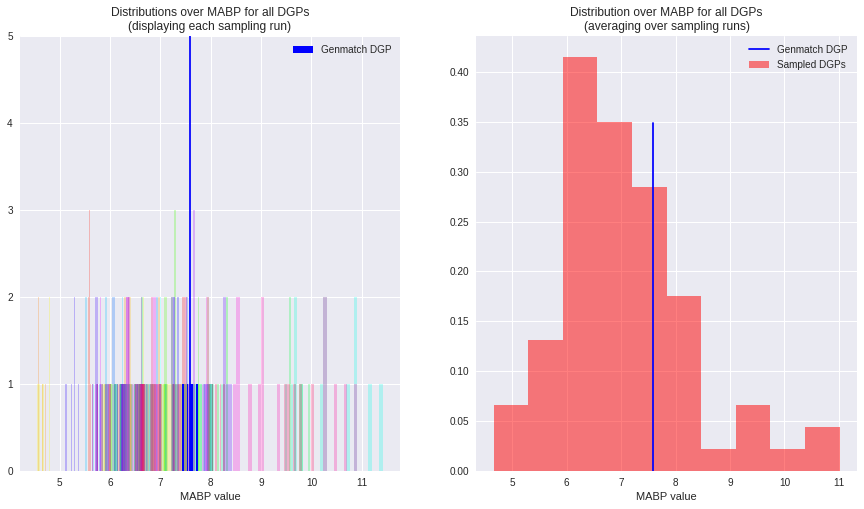
\includegraphics[width=1\linewidth]{figures/ch7-benchmark-pure-synth-1.png}
    \caption{Pure, Synthetic benchmark performance metric comparison. The concrete DGP from the Genmatch paper is a typical sample from a fairly wide distribution over possible performance metrics. Left panel: the distribution over the MABP for each sampling run, for each DGP. Each DGP is in a different color. Right panel: the distribution over the mean value of the performance metric across all sampling runs for each DGP.}
    \label{fig:benchmark-validation-pure-synth-1}
\end{figure}
\FloatBarrier

The natural question to ask at this point is how the performance metrics are correlated to the data metrics. Figure \ref{fig:benchmark-validation-pure-synth-2} shows the MABP performance metric plotted against a metric for treatment nonlinearity. This plot is interesting. Firstly, while there is a clear (and significant, with p=0.0001) correlation, this correlation is reversed from what we would expect. One would expect that as the linearity increases (with higher values of the metric corresponding to increased linearity), the performance of the Logistic Propensity Matching estimator - which estimates propensity scores using a linear model - would improve. However, the reverse appears to be true. This may be because the more linear the function, the more alignment there is between the treatment and outcome functions (the outcome function is linear), and this then means there is a larger degree of confounding to reverse.

\vspace{\baselineskip}

Regardless of the trend direction, there are two important observations.

\begin{enumerate}
    \item Even within a narrow set of functions, there is variance in the position of DGPs in the distributional problem space as measured by data metrics. This variance is significant in that it is meaningfully correlated with changes in the performance of estimators. This means that choosing a single DGP from the set of possible DGPs is risky as it could appear anywhere in the distribution over the possible distributional setting and hence anywhere in the distribution over estimator performance.
    
    \item Even though the data metric is predictive of performance, there is still significant variance in the performance metric at each data metric. This implies that even DGPs with similar measurable distributional settings on one axis may differ in other performance-relevant axes.
\end{enumerate}

Both of these points imply that sampling DGPs to capture, and then average over, the distribution of performance metrics for a given estimator is crucial. Using a single DGP risks picking an arbitrary location in the distribution without any indication of the underlying variance. The first point also motivates an approach that targets specific locations in the distributional problem space by targeting measurable metric values. If these metrics are indeed predictive of performance, then a complete exploration of the performance of an estimator requires exploring its behavior under all and/or known distributional settings.

\begin{figure}[ht!]
    \centering
    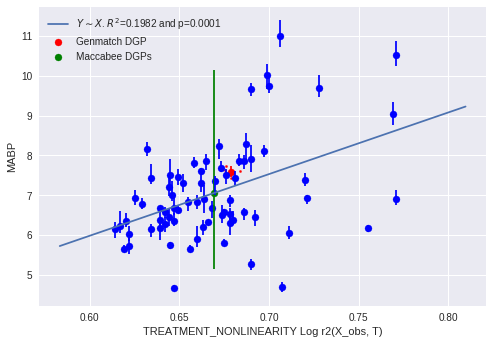
\includegraphics[width=1\linewidth]{figures/ch7-benchmark-pure-synth-2.png}
    \caption{Pure, Synthetic benchmark performance metric plotted against the data metric values for treatment non-linearity. Maccabee sampled DGPs are in blue with a large dot at the mean performance/data metric value for each DGP and error bars corresponding to the standard deviation of the performance metric across sampling runs. Genmatch, concrete DGPs are in red with a large red dot at the the mean performance/data metric value and an individual, smaller dot for the performance/data metric value of each sampling run. It is clear that the treatment non-linearity metric is predictive of performance but only explains a small portion of the variance in the performance. It is also clear that the concrete Genmatch DGP displays performance which is typical of its treatment non-linearity.}
    \label{fig:benchmark-validation-pure-synth-2}
\end{figure}
\FloatBarrier

\subsection{Sampled vs Static Hybrid DGPs}

\textbf{Results for this comparison are pending.}

\subsection{Sampled, Hybrid DGPs vs Empirical DGP}

\textbf{Results for this comparison are pending.}

\end{document}